\documentclass[12pt]{article}
\usepackage{threeparttable}
\usepackage{booktabs}
\usepackage{inputenc, amsmath,amssymb, amsthm}
\usepackage[font=small,labelfont=bf,
   justification=justified,
   format=plain]{caption}
\usepackage{subcaption}
\usepackage{longtable}
\usepackage{adjustbox}
\usepackage{graphicx}
\newtheorem{theorem}{Theorem}
\usepackage{xcolor}
\usepackage{float}
\usepackage[colorlinks=true,
            linkcolor=blue,      % color of internal links (sections, pages, etc)
            citecolor=blue,      % color of citation links
            urlcolor=blue,       % color of URL links
            filecolor=blue]{hyperref}
\usepackage{url}
\usepackage{array}
\usepackage{url}
\usepackage{tikz}
\usetikzlibrary{shapes.geometric, arrows, positioning, fit}
\usetikzlibrary{calc}
\usepackage{titling}
\usepackage{lipsum}
\usepackage{natbib}
\usepackage{setspace}
\usepackage[margin=.75in]{geometry}
\usepackage{xcolor}
\usepackage{amsmath, amssymb, amsfonts}  % loads all AMS symbols & environments

\theoremstyle{definition}
\newtheorem{definition}{Definition}[section]
\usepackage[english]{babel}

\onehalfspacing


\graphicspath{{../../../../../Dropbox/Lawsuits Asymmetry/output}}


\title{Streamlining vs Density Bonuses: \\
 What Drives Affordable Housing Development?}
\author{Tyler Jacobson}
\begin{document}
\maketitle
\section{Motivation and Research Question}

Over the last ten years state and local governments across the United States have attempted to loosen zoning laws in order to increase housing construction and lower prices. California has especially been part of this trend passing something like 100 housing laws since 2016. 

Despite the zoning reform, housing supply in the state has hardly budged. One explanation is that even if larger projects are permissible under zoning law, a developer may not be able to successfully get the approvals they need in order to take advantage of the new law. 

While recent attempts at streamlining permitting and the regulatory approval of new housing may reduce the importance of this mechanism, we do not yet have quantitative evidence on how successful streamlining reform will be. 

In this paper, I ask how difficulties in getting government approval of new housing affect how zoning reform translates into new housing construction. I focus on the city of Los Angeles, which both has excellent data on their approval process and has attempted to reform their housing approval laws. 

I start by documenting facts on the approval process. First, the entitlements process is time-consuming and variable with certain projects having much more difficult review than others. This is a function of realized opposition. Opponents to new housing may challenge approvals via appeals and lawsuits. In addition, the local city council member anecdotally has control over the approval of new housing in their home areas. 

Places where proposed projects face a difficult path toward approval may not be the places where approval is most difficult. Developers anticipate where the entitlements process may be most difficult and forgo proposing projects where they do not expect to succeed in making it through the approval process. I develop a framework where the location of where developers choose to propose projects informs us of their beliefs of the cost of the entitlements process. Combining that with data on the location of opposition to proposed projects, I can characterize where the entitlements process is most difficult. 

In the second part of the paper, I provide evidence that streamlining reform unlocks unsed zoning capacity in the areas with especially large opposition to new housing. I use measure the effects of the ED1 reform to do so. I first show that the reform considerably reduced approval times. Then, I show that the largest increase in proposed housing construction is in the places with the most opposition to new housing. 

One concern with the ED1 policy is that while many projects are proposed, there so far is not a ton of projects actually breaking ground. Linking to building permits, I show that while building conditions are difficult in Los Angeles right now, ED1 projects are completing at higher rates than other comprable approved entitlements. 

\section{Original Motivation}


Local governments concerned with increasing housing affordability are pursuing policy to streamline approval processes epsecially for affordable projects. Today, NYC announced the results of its SPEED task force and is interested in removing things like environmental review from the approval pipeline for affordable housing. Debate over streamlining was central to the housing debate for California gubernatorial candidates. 

Despite interest in pursuing affordable housing review streamlining, there is a dearth of evidence on the potential effects of the policy. In this paper, I study a housing program in Los Angeles, Executive Directive 1 (ED1), that streamlined affordable housing review. The policy quickly had dramatic takeup. Tens of thousands of units entered the affordable housing pipeline. Yet despite the initial takeup, only a fraction of units have broken ground. 

A common feature of many housing policies, ED1 changed multiple facets of development and didn't just streamline. Under ED1, developers were able to propose much larger, and much denser projects under ministerial review than they could have otherwise. This begs the question, were the increase in applications for ED1 driven by the streamlining or the increase in density. 

I begin by measuring the streamlining and density effects. Using administrative data on entitlement applications, I document that ED1 projects moved through entitlements in about half the speed of comparably sized residential projects. Perhaps more importanlty, the frequency of extreme outcomes were considerably reduced under ED1. It is exceptionally rare for an ED1 project to take over a year in entitlement review whereas that is common for non ED1 housing projects. 

The density benefits to developers are also exceptionally large. ED1 proposals tend to add X units compared with what the zoning code allows on similar parcels. 

To assess whether the streamlining or density benefits were quantitatively more important to the decision to apply for the policy, I build a basic model of developer's choice to participate in the program. The key decision variable depends on what the developer could have built absent the program. By quantifying the density benefits, I can ask how large the developer's discount factor would have to be in order for the streamlining benefits to outweight the density benefits. I find that under the standard discount factor of 10\%, the density benefits represent Y\% of the gains of the policy.

\subsection{Literature Review}


The policy did three things. First, it allowed larger projects with smaller units to be built on parcels that previously did not allow that by right. If a developer would have wanted to build according to those dimensions, they would have had to ask for a very specific zoning change in order to make the project feasible. Then, it made it so the project would be approved in a much shorter period of time. How can we think about the incentives to build housing? What were the effects of the policy? To get at the counterfactual, we need to understand what would have been allowed on that parcel of land absent the policy. That involves two things: 1. what was allowed ministerially absent the policy? What did the zoning code allow? 2. What could a developer reasonably have gotten approved under discretionary review without the program? This involves thinking about local opposition and the dynamics of getting approval. This gives us a table for each parcel with three options:

 \begin{figure}[H]
        \centering
        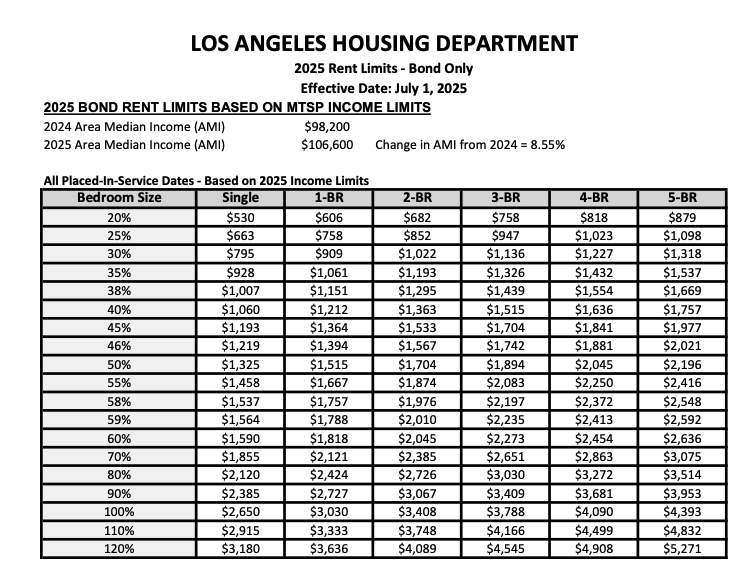
\includegraphics[width=.8\textwidth]{rents.png}
        \caption{Rent Limits in 2025}
\end{figure}


\section{Background on ED1}

\section{Data}
\subsection{Entitlements}
\subsection{Building Permits}
\subsection{Transaction Prices}


\section{Stylized Facts on ED1}
In this section, I document stylized facts on the ED1 program. First, I show that there is considerable takeup of the program. Since 2022 when Mayor Bass launced the program, the majority of entitled housing units are proposed through the program. In addition, the policy takeup is more evenly spread across high and low renter areas compared with the entitlements of other multifamily housing. 

Second, I verify that as promised, the program provides considerable streamlining benefits. ED1 projects are approved considerably quicker than other entitlements of similarly sized projects and there is less of a chance that there are particularly onorous development outcomes. 

Finally, I document that there are considerable density benefits of the program. Historically, the only in areas very close to transit are there high density projects. ED1 projects are high density regardless of where they are proposed within the city. 

In future descriptive work, I hope to show where the ED1 projects are actually likely to be built. 

\subsection{Program Takeup}
Developers took advantage of the policy. Panel B of Figure 1 shows that in 2024, developers proposed more units using ED1 than other kinds of entitlements combined. Overall Y units were added to the affordable housing pipeline. While this was a time period where not many housing units were proposed as there were considerable building hurdles, the sheer numbers of the units proposed suggested that this was a policy worth pursuing. 
\begin{figure}[H]
    \centering
    \begin{subfigure}[b]{0.48\textwidth}
        \centering
        \includegraphics[width=\textwidth]{ed1/ed1_cases.pdf}
        \caption{Total Cases}
    \end{subfigure}
    \hfill
    \begin{subfigure}[b]{0.48\textwidth}
        \centering
        \includegraphics[width=\textwidth]{ed1/ed1_units.pdf}
        \caption{Total Units}
    \end{subfigure}
    \caption{ED1 vs Other Housing Entitlement Proposals}
\end{figure}
Developers may have proposed projects in order to create option value. Getting approval through ED1 need not require developers to build and may even provide bargaining leverage for future development with the city. To assess, the quantitative importance of this story, I link ED1 entitlement applications to permits in LA. Only Z\% of ED1 projects have broken ground suggesting that option value is an important part of the story.  

 \begin{figure}[H]
        \centering
        \includegraphics[width=.8\textwidth]{ed1/ed1_distribution_renter_share.pdf}
        \caption{Distribution of ED1 Units Across Renter Share}
\end{figure}


\subsection{Streamlining Benefits}
How much faster did review go for projects that are ED1 compared to similarly sized projects? Compare both discretion and the full application timeline.

\begin{figure}[H]
    \centering
    \begin{subfigure}[b]{0.48\textwidth}
        \centering
        \includegraphics[width=\textwidth]{ed1/ed1_average_length.pdf}
        \caption{Average Discretionary Case Length Comparison}
    \end{subfigure}
    \hfill
    \begin{subfigure}[b]{0.48\textwidth}
        \centering
        \includegraphics[width=\textwidth]{ed1/ed1_share_above_365.pdf}
        \caption{Likelihood of Extreme Outcome}
    \end{subfigure}
    \caption{ED1 Streamlining Benefits}
\end{figure}


\subsection{Density Benefits}
Take all the ED1 parcels: use the zoning code to and characteristics of the land to predict what would have been built. What is the difference in square footage and what is the difference in unit counts?


 \begin{figure}[H]
        \centering
        \includegraphics[width=.8\textwidth]{ed1/ed1_size_transit.pdf}
        \caption{Units Per 1000 SqFt of Land}
\end{figure}

\subsection{What is Actually Built?}
ED1 is frequently critized as not actually leading to many housing units being built. This is certainly true. The following figure shows that the number of ED1 units with a matched building permit is far below the number of proposed units. However, what is underappreciated is that this is mostly a function of Los Angeles not building at the moment. The figure below shows that ED1 projects are actually more likely to be built than other comparably sized projects that are approved around the same time. 
 \begin{figure}[H]
        \centering
        \includegraphics[width=.8\textwidth]{ed1/ed1_matched_permits.pdf}
        \caption{Fraction of ED1 Projects with Building Permits}
\end{figure}

 \begin{figure}[H]
        \centering
        \includegraphics[width=.8\textwidth]{ed1/ed1_matched_permits_binscatter.pdf}
        \caption{Built ED1 Projects vs Other Entitlements}
\end{figure}


\subsection{From Stylized Facts to New Knowledge}
In this section, I show clearly that the ED1 program had strong takeup (even if not many projects are actually built), and that program timelines are considerably shorter and developers ask for larger projects. 

ED1 did nothing to change the zoning code or modify what developers are able to ask for. For that reason, it's clear that regulatory streamlining can induce the proposals of projects that otherwise would not have been worth proposing even if they are compliant with the zoning code. The general lesson is that what is possible to get approved via the entitlements process is important. Strong evidence of the such would be to have a measure of whether building is especially difficult and show that ED1 unlocks that building potential.  


\newpage
\appendix
\section{Regulatory Texts}
\subsection{Original Text of ED1}
    
To aid in swiftly sheltering people who are unhoused in the City of Los Angeles, and by virtue of the authority vested in me as Mayor of the City of Los Angeles under Section 231(i) of the Los Angeles City Charter and the provisions of Section 8.29 of the Los Angeles Administrative Code, I hereby declare the following order to be necessary for the protection of life and property and I hereby order, effective immediately, that:

1. Applications for 100\% affordable housing projects, or for Shelter as defined in Section 12.03 of the Los Angeles Municipal Code (LAMC) (hereinafter referred to as Shelter), shall be, and hereby are deemed exempt from discretionary review processes otherwise required by either the zoning provisions of Chapter 1 of the LAMC or other Project Review including Site Plan Review as described in LAMC Section 16.05 and LAMC Section 13B.2.4, as long as such plans do not require any zoning change, variance, or General Plan amendment. All City departments are directed to process all plans for such 100 percent affordable housing projects or Shelter using the streamlined ministerial review process currently used for projects eligible under Government Code section 65913.4, State Density Bonus law.   

2. An application for the development of a 100 percent affordable housing project or Shelter may use the density permitted for that site either by the applicable zoning or the General Plan Land Use Designation, consistent with state law. In addition, a project may utilize the State Density Bonus and LAMC bonuses, incentives, waivers and concessions if such are in compliance with the applicable requirements. 

3. I further direct all applicable City Departments to process clearances and utility releases related to building permit applications, certificates of occupancy, or temporary certificates of occupancy within 5 business days for 100 percent affordable housing projects and within 2 business days for Shelters. 

4. I further direct all applicable City Departments to conduct and conclude all reviews and inspections required for 100 percent affordable housing projects or Shelters and to issue all appropriate approvals for such projects or Shelters within 60 days following the submission of the completed application. City Departments shall provide the applicant with all required changes or amendments on or before the 30th day following the submission of a completed application for such projects. To the extent practicable, all required reviews and approvals shall be conducted simultaneously, not sequentially, by all City departments so as to meet the 30 day and 60 day periods specified for such projects in this paragraph. 

5. I hereby direct the Los Angeles Housing Department (LAHD) to coordinate with the Los Angeles City Controller to track and process all affordable housing projects and expedite payments thereon. LAHD shall track each pending pay application, initial submittal date, approval date, reasons for rejection or modification of submitted payment applications, and issuance of payment, and shall provide reports to the Mayor on all such payments at least monthly with the goal of expediting payments due for affordable housing projects.

6. I hereby direct that all protocols set by the Los Angeles County Coordinated Entry System as they apply within the City of Los Angeles be expanded, changed, or suspended, as allowed by federal law.  Rules, guidelines and regulations will be developed to expedite the placement of unhoused neighbors into housing in the City of Los Angeles. 

7. I hereby direct all City departments to prioritize and streamline compliance with the provisions of the Building Homes and Jobs Act – Government Code section 27388.1 in order to maximize the City’s eligibility for state and federal funds to support the development of emergency shelters, transitional housing, and supportive housing. The City shall seek to comply with or otherwise meet all criteria specified under all applicable state and federal laws that provide for increased resources, funding, access or allowance for temporary or affordable housing.

8. Effective February 28, 2023, in accordance with the end of the State of California COVID-19 emergency, I hereby rescind the Public Order Under City of Los Angeles Emergency Authority issued on January 28, 2022 (January 28, 2022 Order).  Notwithstanding this action, all entitlements already approved and still valid as of this date, or approved during the effective period of the January 28, 2022 Order, shall remain valid for the extended time period(s) as if such January 28, 2022 Order were still in effect with respect to such entitlements.  Furthermore, local decision-makers, including the Director of Planning and the Chief Zoning Administrator, are authorized to continue to hold all required public hearings under the Los Angeles Municipal Code in a manner consistent with the Governor’s Executive Order N-29-20, and any subsequent orders or published guidance pertaining to local legislative bodies. 

9.       The City Planning and Housing Departments shall issue guidelines as necessary to implement the provisions of this Executive Directive. 

\subsection{State Density Bonus Law}
\textbf{The key provision of State Density Bonus Law applying to ED1}

(D) For housing developments meeting the criteria of subparagraph (G) of paragraph (1) of subdivision (b), the following shall apply:

(i) Except as otherwise provided in clauses (ii) and (iii), the density bonus shall be 80 percent of the number of units for lower income households.

(ii) If the housing development is located within one-half mile of a major transit stop, the city, county, or city and county shall not impose any maximum controls on density.

(iii) If the housing development is located in a very low vehicle travel area within a designated county, the city, county, or city and county shall not impose any maximum controls on density.

\textbf{What is subparagraph (G) of paragraph (1) of subdivision (b)?}

(G) One hundred percent of all units in the development, including total units and density bonus units, but exclusive of a manager’s unit or units, are for lower income households, as defined by Section 50079.5 of the Health and Safety Code, except that up to 20 percent of the units in the development, including total units and density bonus units, may be for moderate-income households, as defined in Section 50053 of the Health and Safety Code. For purposes of this subparagraph, “development” includes a shared housing building development.

\end{document}


\section{Affordable vs Market Rate Rents}
ED1 projects are 100\% affordable, which reduces their market value compared to traditional market rate projects. How much less valuable are these projects than comparable market rate projects? To assess this, I use the entitlements data to link the number of affordable units to real estate transactions. I then run the following regression:

$$\ln P_j = \theta_t + \gamma_n + X'_j\beta + \delta aff_j + \epsilon_j$$
where $j$ is a parcel, $t$ is the year of sale, $n$ is the tract, $size_j$ is the size of project, and $aff_j$ is the share of units in that building that are affordable.  

We expect the affordability penalty to be largest in areas that 

\section{ED1's Effect}
This section lays out how I think about the effect of the ED1 program on both the profitability of the allowed building envelopes and the benefits of streamlining. Absent ED1, a developer can follow two pathways: by-right and discretionary. By-right projects are ministerial in nature and are approved unless the developer makes a mistake. Discretionary projects follow a longer review process with uncertainty over approval and legal status\footnote{Certainly a developer could build far beyond the zoning threshold. For now we ignore that option and consider. These are rare these days.}. 

\subsection{By-Right Absent ED1}
By-right projects building envelope is defined by a few regulations:
\begin{itemize}
    \item Height restrictions: the max height or FAR that a building can have according to its zoning code
    \item Density restrictions: each zoning code will have a maximum number of units per square foot
    \item Lot size restrictions: each multifamily zoning code has a minimum lot size that must be hit before the policy can be applicable.
\end{itemize}


\subsection{Original ED1 Policy}
The original ED1 policy contained the following provisions:
\begin{enumerate}
    \item 100 percent projects are ministerial as long as they do not require a zoning change
    \item An application may use the density required under either the zoning or the general plan. They may use density bonuses under statewide density bonus law and LAMC. The key thing here is that for projects within a half mile of transit, there is no limited on maximum density. 
    \item Clearances, Reviews, and inspections are directed to go more quickly. 
\end{enumerate}
Basically the intention of the policy was to make ministerial what previously was considered to be discretionary. The policy does nothing to change what the allowed envelope of buildings could be. There were already existing laws that gave certain density bonuses to 100 percent affordable projects. These projects may however have been encumbered by the discretionary process. It seems like there is a distinction to be made between what can be approved and the costs of getting those projects approved. ED1 both lowers the costs of going through the approval process and also allows larger projects to be approved. The challenge is that these things are correlated. 

How does permitting streamlining and removing discretionary review affect the effects of zoning policy? Los Angeles and the state of California have attempted to increase the zoning envelope for projects. There are policies that increase allowed density near transit, and for affordable housing projects. In Los Angeles, the effects of these laws are potentially mitigated by the permitting system. Despire recent attempts at permitting reform, we do not have empirical evidence on the effects of these laws. 


\subsection{Example of ED1 Project}

\section{Testing for Differential Effect in Transit Areas}
A key aspect of the ED1 policy is that it allows for unlimitted density in areas within a half mile of transit. If this unlimitted density unlocks projects, there should be a large treatment effect at this threshold. 

$$Y_j = \beta_0 + \beta_1 D_j + \delta 1\{D_j<.5\} + \epsilon_j$$

where $Y_j$ is whether the parcel has an ED1 application on it and $D_j$ is the distance to transit. 



\section{Framework}



Value of building a project with characteristic $X$:
$$A(X)\beta^{T(X)}\pi(X)-F(X)$$

The project has approval likelihood, $A(X)$, time to approve/build $T(X)$, profits $\pi(X)$ and upfront cost $F(X)$. 

ED1: ED1 allows a certain max density $X^{ed1}$
\begin{itemize}
    \item $A(X^{ed1}) = 1$: ED1 is ministerial so guaranteed to be approved along as you follow the rules
    \item $T(X^{ed1})$: as we can see above the project approval timeline is considerably shortened
    \item $\pi(X^{ed1})$ density is increased but revenue from building is less because of the affordability requirements. 
\end{itemize}

\subsection{Linear + Fixed Costs}
Let $\pi(x)=(p-c)x-F$
so there is a fixed cost of building housing and then a linear return to building more units. Here, the developer would like to build as large as possible. 
Under ED1, the developer can build $x^{ed1}=x^{br}(1+\gamma)$ but must receive $\tau$ of the normal rents. The density benefits from ED1 compared to another affordable housing project are:
$$(p-c)(1+\gamma)$$
The higher the affordable return relative to the cost of building an additional unit, the higher the benefit of the ED1 density. 

Compared to a by-right project, we need to think about not just the change in density but also the change in profits:

$$(\tau p - c) x^{br}(1+\gamma) - (p - c) x^{br}$$
So now, in places with higher rents, the density benefits are going to be less because of the penalty of the affordable housing. 

\subsection{Streamlining Benefits}
Imagine we have calculated the value of an ED1 project and the value of a market rate project:
$$\pi^{ed1}(x_j), \pi^{market}(r_j, x_j)$$
Call the streamlining benefit: $S$
Then the developer chooses ED1 if:
$$\pi^{ed1}(x_j)+S>\pi^{market}(r_j, x_j)$$
We can use this inequality to construct bounds on the streamlining benefits. Any time the developer chooses the market rate project, we know the streamlining benefits cannot be large enough to overcome the difference. Any time the developer chooses ED1 when the return to doing so is negative, we know the streamlining benefits outweigh the decline in value from building according to ED1. 

In places that are high rent, we might expect the ED1 project to be lower value than the market rate project. If we saw that these ED1 projects were being chosen, that would suggest that the streamlining benefits of the ED1 program are large. We probably will not observe many ED1 projects being chosen over market rate projects--there probably are not many market rate projects being built at the same time because of the decline in building in Los Angeles over this period. 

\section{Proposal Choice}
Where might we expect ED1 to have the largest proposal effect?
\begin{enumerate}
    \item In places with low rents, the higher the rents, the more the developer gives up by building affordable housing. 
    \item In places where the density benefits are largest. In TOC areas, the effect of the density bonus is largest. 
\end{enumerate}

\section{Doubts and Next Steps}
\begin{enumerate}
    \item Not that many ED1 projects are built 
    \item Not that many non Ed1 projects are built over this period making it difficult to construct the bounding exercise. 
    \item How well can I actually estimate the return to building? What is the quickest way to doing that?
\end{enumerate}
Next steps:
\begin{enumerate}
    \item Link to building permits and ask how many Ed1 projects have actually broken ground
    \item For the ED1 projects that have broken ground what do they look like? What is cost per unit compared to other affordable housing projects?
    \item How much bigger are ED1 projects than what can be built by right?
\end{enumerate}